%# -*- coding: utf-8-unix -*-
%%==================================================
%% chapter01.tex for SJTU Master Thesis
%%==================================================

\algnewcommand\algorithmicforeach{\textbf{for each}}
\algdef{S}[FOR]{ForEach}[1]{\algorithmicforeach\ #1\ \algorithmicdo}
%\bibliographystyle{sjtu2}%[此处用于每章都生产参考文献]
\chapter{系统设计}\label{chap:sys_design}
\section{容器云相关技术分析}
\subsection{Docker镜像}
Docker镜像是Docker容器运行的基础,提供了运行容器所需要的依赖环境和环境配置。Docker镜像本身基于分层文件系统,将所有的文件变化和环境配置变更都作为内部文件系统层级的变更,本质上是一个包含着一系列文件系统层级修改的有序集合\footnote{https://docs.docker.com/glossary/?term=image}。由于Docker容器利用了写入时复制(copy-on-write,CoW)作为容器内部分层式文件系统读写策略,基于同一Docker镜像创建的不同容器实例可以共享这个镜像底层的文件系统,这也大大方便了Docker镜像的制作。因此,Docker用户常常会引用其他基础镜像作为自身镜像的基础。

\begin{table}[h]
\centering
\bicaption[tb:dist_size]{不同Linux发行版本镜像在最受欢迎应用镜像中引用的分布情况}{不同Linux发行版本镜像在最受欢迎应用镜像中引用的分布情况}{Table}{Linux Distribution Images References In Most Popular 30 Application Images on Docker Hub}
\begin{tabular}{@{}llrr@{}}\toprule
 发行版本 & 版本代号 & Docker镜像大小(MB) & 引用计数 \\ \midrule
 Debian & Jessie & 123 & 25\\
 Ubuntu & Xenial & 119 & 3\\
 Alpine & 3.6 & 5 & 2\\ \bottomrule
\end{tabular}
\end{table}

除此之外,Docker在1.10版本之后引入了内容寻址功能,使得Docker镜像中的同一文件层级在不同机器和实例中都有相同的唯一标识,大大方便了Docker容器在不同环境下的迁移\footnote{https://github.com/moby/moby/wiki/Engine-v1.10.0-content-addressability-migration}。这个新的特性使得即使是基于不同Docker镜像构建的容器也能共享底层的部分共用镜像,比如相同的操作系统镜像和运行时环境等。为了调查不同镜像在底层基础镜像上的共享情况,我们在目前最受欢迎的容器镜像仓库,同时也是官方镜像仓库Docker Hub\footnote{https://hub.docker.com/}上对当前最流行的30个应用镜像进行调查,得到的统计结果如表\ref{tb:dist_size}所示。由表\ref{tb:dist_size}可知,大量的应用镜像依赖于少数几种底层基础镜像。考虑到对网络流量和存储空间的影响,这些基础镜像的大小是很重要的。尽管用户可以选择基于\emph{Alpine}或者\emph{scratch}这类更小的镜像来制作容器镜像,但是由于诸如\emph{Debian} 或者\emph{Ubuntu}等Linux发行版本通常默认自带诸如\emph{apt}和\emph{wget}等有用的工具而且环境设置更友好,大家还是更喜欢使用这些自己更熟悉的Linux发行版本来管理依赖环境和环境配置。

\subsection{已有的容器集群管理框架}
\begin{figure}[htbp]
\centering
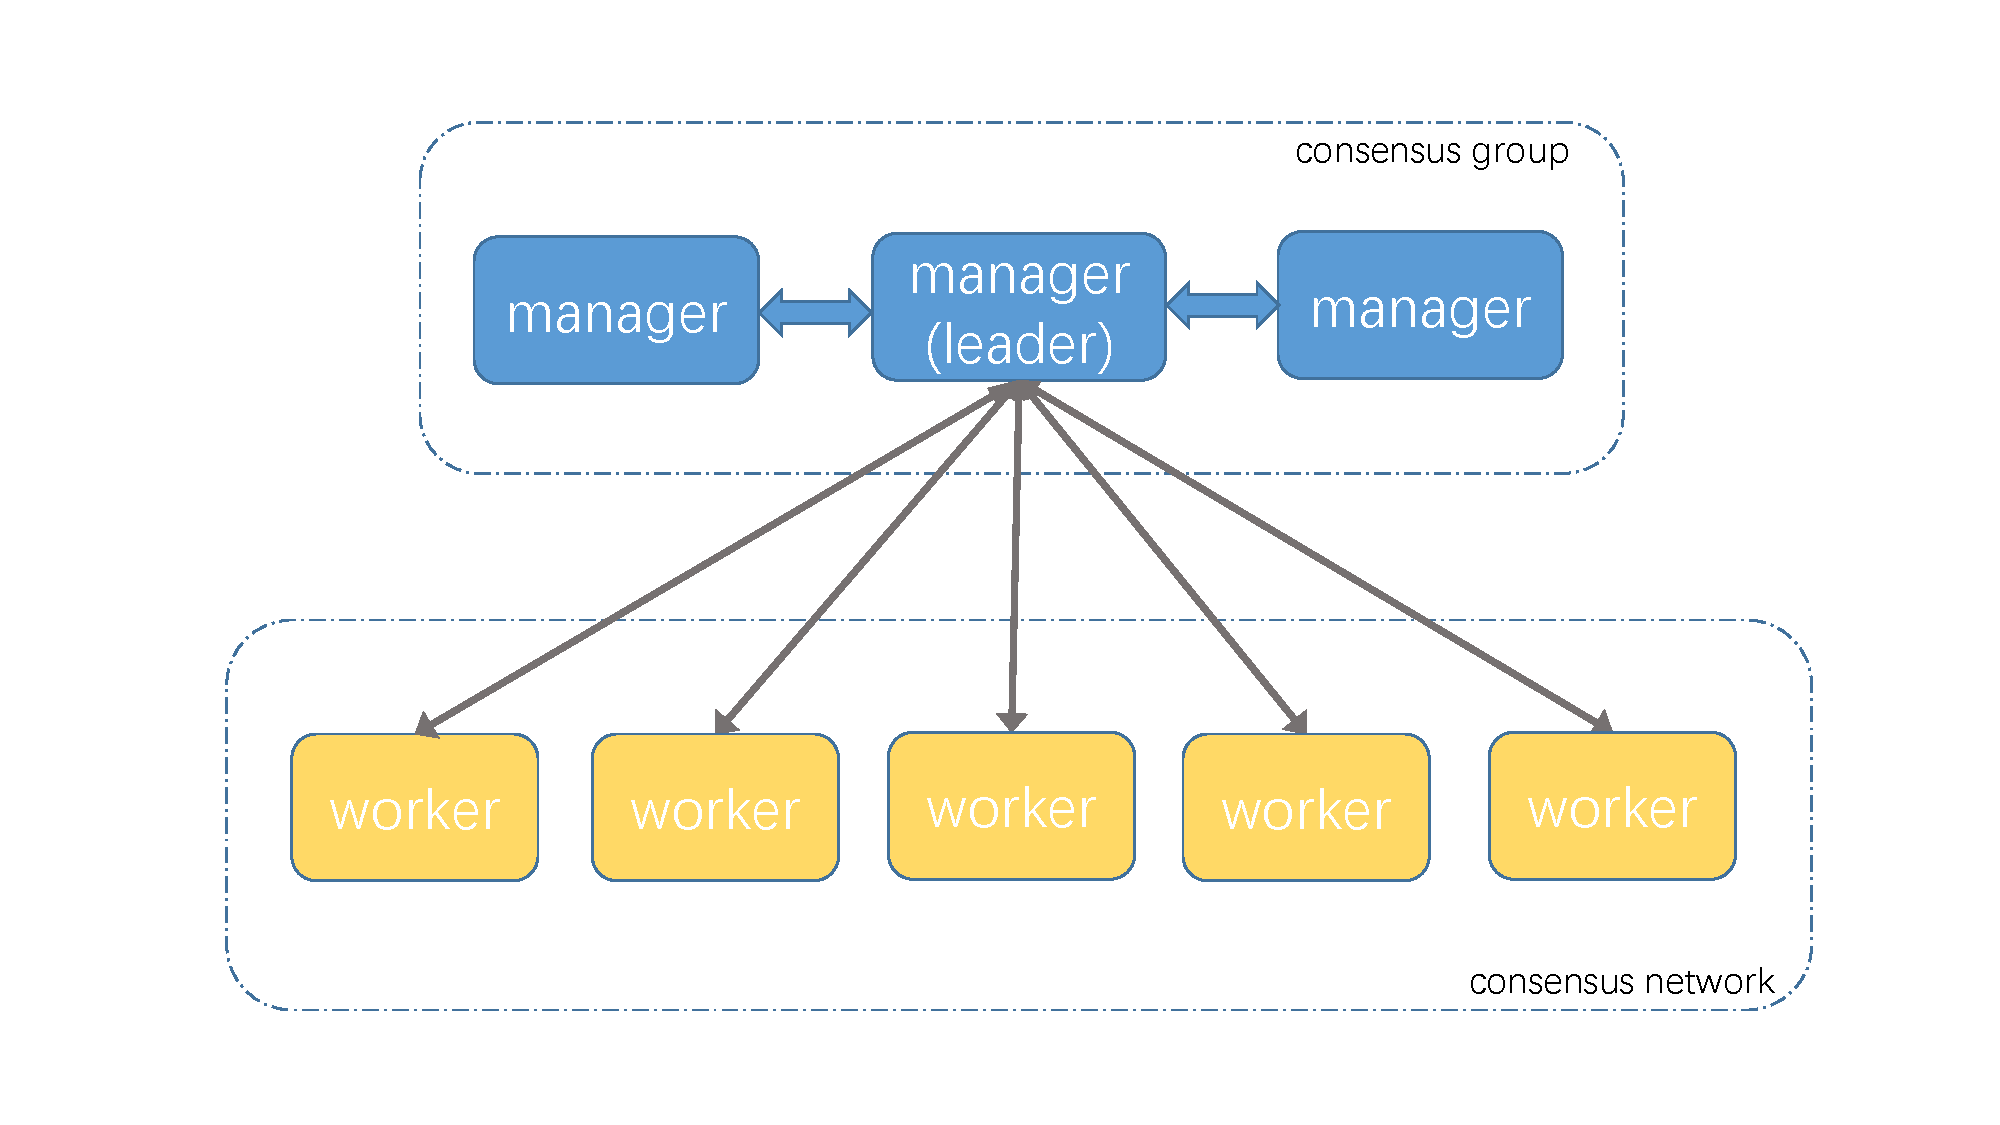
\includegraphics[width=0.9\textwidth]{./figure/manager-worker}
\bicaption[fig:manager-worker]{集群的分布式系统架构}{\textbf{集群的分布式系统架构}}{Fig}{Architecture in Container Cluster}
\end{figure}
当前主流的容器集群管理框架都是基于分布式系统架构进行设计,将每个物理服务器作为集群中的节点来构建分布式的集群。如图\ref{fig:manager-worker}所示,在当前主流的容器集群框架设计中,集群中的节点分为两类:管理者节点和工作者节点。管理者节点之间通过诸如paxos和raft等一致性协议构建一致性群组,从而实现容器集群中管理者功能的高可用;工作者节点基于gossip等一致性协议构建一致性网络,保证数据在工作者节点之间的一致性;管理者节点按照所选择的一致性协议周期性地从所有管理者节点中选择出领导者节点,领导者节点和工作者节点之间进行通信并将数据同步给其他的管理者节点。

目前构建容器云常用的框架主要有Docker Swarm、Kubernetes和Mesos,其中Docker在1.12版本之后引入了swarmkit作为原生的swarm mode提供了默认的Docker容器集群支持,这三者针对负载变化的场景均只能通过修改副本数的方式来进行容量调整。在独立的Docker Swarm中,提供三个不同的调度策略供用户选择:\emph{spread}模式,\emph{binpack}模式和\emph{random}模式。其中,\emph{spread}模式将任务平均分配到集群中所有的节点上;\emph{binpack}模式则恰恰相反,使用贪心算法将任务分配到当前可以选择的任务最多的节点上,优先将集群中的节点按照装箱的方式依次装满;\emph{binpack}模式则先筛选符合条件的集群节点,然后将任务随机的分配到其中的一个节点上。在Docker swarm mode中,目前只支持和\emph{spread}模式分配思路一样的\emph{SpreadOver}模式。Kubernetes则通过插件的方式提供多种调度模式的支持,包括但不限于按节点资源使用量均分、按节点任务数均分、资源利用率最高的节点优先和资源利用率最低的节点优先等,其中也支持将使用相同镜像的容器聚集的模式,但是要求必须是同一个容器镜像。Mesos则作为一个分布式资源框架,要求用户自己实现调度器或者使用诸如Marathon\footnote{https://mesosphere.github.io/marathon}等第三方调度框架,默认不提供任何负载均衡和资源调度的支持。综上而言,目前已有的各个容器调度框架没有针对可用性和负载变化进行区分,没有默认的服务可用性支持,需要用户手动控制副本数以满足服务的可用性,通过变更服务的副本数来应对负载的变化;各框架更多的关注于提升整体资源利用率,而忽视了服务可用性和服务容量变化成本之间的平衡。

\section{系统架构}
本课题以资源使用率作为实际负载的衡量标准,提出基于容器的主动式容器云负载优化模型,旨在在负载多变的场景下,加速容器云中服务对负载变化的响应,加强容器云对负载变化的灵活性,从而更好的应对负载,提升容器云整体的服务质量。模型的整体架构设计如图\ref{fig:sys_design}所示,一共分为资源使用状态监测、资源使用状态预测、资源供给方案生成、资源供给优化、资源管理和负载均衡等6 个模块。由于应用于容器云这一分布式的架构环境中,本课题提出的模型中各模块也将基于分布式架构的思想来设计,以提升整体模型的性能和可靠性。
\begin{figure}[htbp]
\centering
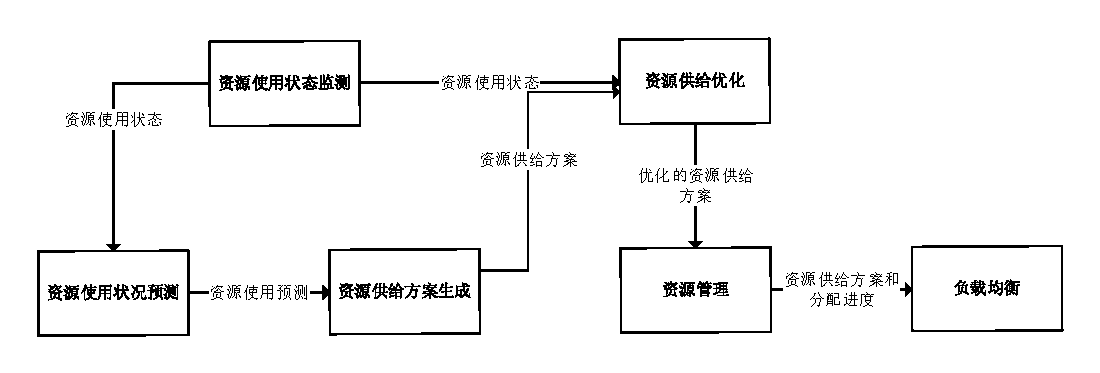
\includegraphics[width=0.9\textwidth]{./figure/sys_design}
\bicaption[fig:sys_design]{系统架构设计}{\textbf{系统架构设计}}{Fig}{System Architecture}
\end{figure}

我们将整个模型框架分为三个部分:负载监测和预测、资源供给和管理以及负载应对。其中,负载监测和预测部分包括了架构设计中的资源使用状态监测模块和资源使用状态预测模块;资源供给和管理部分包含了资源供给方案生成模块、资源供给优化模块和资源管理模块;负载应对部分则包括了负载优化模块。其中,资源供给和管理部分主要负责对本系统内服务资源的使用状态进行监测并给予历史监测数据给出未来一段时间内的资源使用预测;资源供给和管理部分基于可用性分析,根据预测的资源使用量和实际的监测状态得到需要的任务实例数目;负载应对部分则依据当前容器云中所有节点的状态和目标服务的限制通过服务伸缩的操作选择合适的节点来托管相应任务实例,从而达到更好的应对负载变化的目标。由于本模型应用于容器云中,所以本质上是一个分布式框架,很多模块利用消息队列通过周期性的异步操作来提升整体的吞吐量,提高框架的整体性能。本文接下来将分别对这三部分进行说明从而介绍整个架构中各模块的设计和涉及的核心技术及算法。

\section{负载监测和预测}
\subsection{资源使用状态监测模块}\label{sec:monitor}
资源使用状态常常随着负载的变化而变化,当负载上升时,相应资源的使用量会相应的增加;当负载下降时,对应资源的使用量则会相对的减少。通过对负载的实时监测,我们可以及时把握负载的状态,并根据负载的变化对服务进行相应的调整,保证服务质量的同时降低成本。同时,对负载的实时记录可以作为原始数据,通过预测等方法进一步的提升服务质量,降低成本。在本课题中,我们用系统中资源的使用状态来表征当时的负载状态,对资源的使用状态进行周期性的监控,并将观测到的结果按照时序数据的格式记录下来。在容器云中,可使用资源的种类可分为以下4 种:CPU、内存、磁盘存储和网络带宽。但是考虑到在目前的主流容器云和管理框架中,主要使用诸如AWS的Amazon Simple Storage Service(S3)等云存储服务,很少使用对应节点上的物理硬盘,我们在本课题中监测的资源类型包括:CPU使用状态、内存使用状态和网络带宽使用状态。容器云本身是一个分布式架构,因此我们通过在容器云中各节点上对各节点本身以及运行在节点上各个任务实例的资源使用状态进行监测,并通过心跳包的传输方式周期性地向容器云中的管理者节点同步各任务实例的资源使用状态和作为集群节点的物理服务器的资源使用状态。为了后续方便后续预测的处理,我们使用时间序列数据的格式来保存监控到的资源使用状态,具体的数据格式如公式\ref{eq:res_format}所示:
\begin{equation}\label{eq:res_format}
\{time, (cu, ca, mu, ma, niu, nia, nou, noa)\}
\end{equation}

在公式\ref{eq:res_format}中,$time$表示该次监测操作的时间点,按Unix时间戳的格式记录,即该时间点到1970年1月1日0点正的毫秒数;$cu$表示此次监测观测到的已使用CPU个数,$ca$表示被监控对象可用的CPU个数,单位均为一个标准CPU核;$mu$表示本次监测观测到的内存使用大小,$ma$代表被监控对象可用的内存大小,单位均为字节(即Byte);$niu$表示本次监测中观测到的网络接收速度,$nia$表示被监控对象的最大可用网络接收速度,$nou$表示本次监测中观测到的网络发送速度,$noa$表示被监控对象的最大可用网络发送速度,单位均为bps。由于网络的发送/接受速度无法通过已有的接口直接获取,必须基于计算两次监控间隔之间发送/接受网络包数量的差值进行计算,计算方法如公式\ref{eq:net_speed}所示:
\begin{equation}\label{eq:net_speed}
networkSpeed_t = \frac{packageSize_t-packageSize_{t-1}}{time_t-time_{t-1}}
\end{equation}
其中,$packageSize_t$表示此次监控观测$t$时刻的网络数据包大小,$packageSize_{t-1}$表示上一次监控${t-1}$时刻观测的网络数据包大小,$time_t-time_{t-1}$表示这两个监控时刻之间的时间差。

资源使用状态监测模块默认每隔100ms对资源使用状态进行一次采集,并且每隔30秒将该时段内的监控数据从各个工作者节点同步管理者节点。每次采集时,除了资源使用状态的信息之外,资源使用状态监测模块还会根据监测对象的类型追加其他的标记数据:如果监测的是集群节点,则标记该数据为节点类型并在资源使用状态数据后追加集群节点的ID;如果监测的是任务实例,则标记该数据为任务实例类型并在资源使用状态数据后追加任务实例的ID和相应服务的ID。在同步之前,资源使用状态监测模块会对采集到的原始监控数据进行预处理,通过对每个时间段内的数据取均值后作为这段时间内的观测数据,以减小短时间内观测值的波动,降低整体的观测误差和传输的数据大小,这个时间段默认为3秒。通过标准化所有监控数据的时间记录点,使得所有节点上报的监控数据中采样时间点一致,从而可以获得集群中所有节点和服务在相应时刻的状态。

\subsection{资源使用状态预测模块}\label{sec:prediction}
目前的框架和容器云均是在资源使用量达到指定阈值后按照诸如实例数翻倍等特定规则进行的自动伸缩。但是在不同的负载场景下使用相同的规则会出现很多问题。以实例翻倍的伸缩策略为例,在负载急剧增加的场景下,按照实例翻倍的策略进行一次调节后仍然不能满足负载的需要,必须通过多次调节才能满足负载的变化。但这就造成了相应延迟,并降低了这一阶段内的服务质量。而在负载增长缓慢的场景下,实例数量翻倍后虽然满足了负载的需要,但是多分配了额外的资源,增加了成本。因此通过可靠的方法对将来的负载状态进行预测,从而可以获知应对相应负载所需要的资源,能更好地保证容器云中的服务质量,降低整体的成本。在本课题提出的模型中,资源使用状态预测模块周期性的对之后一段时间内的资源使用量进行预测。资源使用状态监测模块获得历史监测数据后会将相应数据周期性地给资源使用状态预测模块,默认周期为5分钟。由于资源使用状态监测模块能够提供的最新数据是来自前一个周期的资源使用状态数据,而预测操作本身需要耗费时间,因此在资源使用状态预测模块中对当前周期进行预测显然会造成相应的延迟。为此资源使用状态预测模块根据当前所属周期t之前获得的历史监测数据,利用相应的预测算法对再下一个周期t+1内的资源使用量进行预测。即在默认情况下,资源使用状态预测模块会通过预测算法预测从5分钟之后开始到10分钟之后这个5分钟时间段内服务所需要的资源使用状态,预测结果的数据格式如公式\ref{eq:pred_format}所示:
\begin{equation}\label{eq:pred_format}
\{time, (cu, mu, niu, nou)\}
\end{equation}
其中中,$time$表示下一个周期开始的时间,按Unix时间戳的格式记录,即该时间点到1970年1月1日0点正的毫秒数;$cu$表示预测要使用的CPU个数,单位均为一个标准CPU核;$mu$表示本次预测得到的内存使用大小,单位均为字节(即Byte);$niu$和$nou$分别表示预测要使用的网络接收速度和网络发送速度,单位均为bps。

目前主流的预测方法主要分为基于经典时间序列理论的预测方法和基于人工智能的预测方法两大种类,两类算法各有优缺点:基于经典时间序列理论的预测方法速度更快,但是更多表现为预测结果相对于实际结果的延迟,预测精度较低并且预测值准确度和周期参数设置紧密相关,更加适用于有明显周期性的数据;基于人工智能的预测算法需要额外的数据训练过程,但是由于除了时间特征之外可以加入业务相关特征,因此预测准确性更高。我们引入了预测正确率等预测模型评估标准来帮助我们评估预测模型在容器云环境下的预测准确性和预测结果对后续调整的影响。我们在资源使用状态预测模块中引入了经典时间序列理论的预测算法模块和基于人工智能的预测算法模块供用户选择使用,分别选择基于整合移动平均自回归模型的预测算法和基于长短期记忆模型\cite{hochreiter1997long}的预测算法作为基于经典时间序列理论的预测算法默认实现和基于人工智能的预测算法默认实现。

最后,我们使用开源的98年世界杯网站流量数据\cite{arlitt2000workload}作为用户请求的模拟数据,并且假定每次请求消耗相同的资源和CPU时间。在接下来的几节中,我们将分别对预测模型评估标准进行介绍,并对使用基于整合移动平均自回归平均模型预测算法和基于长短期记忆模型预测算法作为默认预测算法实现的原因进行分析和讨论。

\subsubsection{预测模型评估标准}
在实际中,预测结果往往并不是十分准确,但是我们可以通过在依赖预测结果的基础上根据实际状态进行再次调整的方式来提高系统整体的灵活性,从而进一步地提升系统对负载变化的应对能力。如果预测结果比实际需要的资源总量低,那就导致基于预测分配的资源不足以应付实际的负载,降低整体的服务质量;如果预测结果高于实际需要的资源总量,虽然存在资源的浪费但保证了服务的稳定可用,保障了服务的质量。除此之外,根据Google对Borg的使用分析,在容器云中创建容器的延迟远远比预期的更加严重\cite{verma2015large}。因此,为了更好地响应负载变化,我们自然希望尽量是通过收缩的方式来实现对服务实例规模的调整。为了客观评估预测算法对实际调整的影响,我们在评估容器云中的预测算法效果时引入了预测正确率这一概念,预测正确率计算方法如公式\ref{eq:correctness}:
\begin{equation}\label{eq:correctness}
Correctness_{algo} = \frac{Count(Usage_{predication} >= Usage_{actual})}{Count(Usage_{actual})}
\end{equation}
从公式\ref{eq:correctness}中可以很明显地发现,预测算法可以通过增加自身预测值的方法来提升自身的预测正确率。在保证尽量在预测的结果进行收缩的方式来调整服务实例规模的基础上,我们依然希望相应预测算法能尽量减少预测偏差,从而尽可能的减少资源的浪费。我们引入了预测偏差率$\overline{ME}$和预测偏方差率$\overline{MSE}$来量化地表示预测结果和实际观测值之间的差距,预测偏差率$\overline{ME}$可以量化地表征预测算法的准确性,而预测偏方差率$\overline{MSE}$则可以用量化的方式来表征预测算法预测结果的稳定性,详细计算方法分别如公式\ref{eq:algo_error}和公式\ref{eq:algo_mse}所示:
\begin{equation}\label{eq:algo_error}
\overline{ME_{algo}} = \frac{\sum_{time \in period} {\frac{\vert Usage_{predication_{time}} - Usage_{actual_{time}}\vert}{Usage_{actual_{time}}}}}{Count(time)}
\end{equation}
\begin{equation}\label{eq:algo_mse}
\overline{MSE_{algo}} = \frac{\sum_{time \in period} {\frac{\vert Usage_{predication_{time}}^{2} - Usage_{actual_{time}}^{2}\vert}{Usage_{actual_{time}}^{2}}}}{Count(time)}
\end{equation}

\subsubsection{基于整合移动平均自回归模型的预测算法}
整合移动平均自回归(ARIMA)模型作为经典时间序列预测理论的代表模型,通过对一段时间内的历史数据进行分析从而计算出接下来周期内的预测值。对于有明显周期性质的时间序列数据而言,整合移动平均自回归模型的预测过程更加直观并且准确率较高,在诸如如金融证券市场等具有明显周期性的应用场景中被广泛应用。整合移动平均自回归模型可以看作是一个包含了自回归模型和滑动平均模型的结合,通过差分的方式对时序数据平稳化,利用自回归模型的特性来记录历史值对当前的影响,通过滑动平均模型来描述累积的误差影响。

\subsubsection{基于长短期记忆模型的预测算法}
时间递归神经网络(RNN,Recurrent Nerual Networks)模型通过引入循环的方式使得神经网络中的信息可以持久化\cite{graves2012supervised},因此时间递归神经网络模型很适合应用于时序数据这一具有明显时间依赖的场景中。相比于基于经典时间序列理论的预测算法,基于时间递归神经网络模型的模型除了时间序列本身的特征外还能引入其他业务特性来标记时间序列本身的状态,从而加强模型的表征能力,提高预测精度。但是传统的时间递归神经网络模型很难解决长期依赖的问题:要训练过程中的计算量随着记忆的历史数据增加呈指数型增长\cite{bengio1994learning}。长短期记忆(LSTM,Long Short-Term Memory)模型作为一种时间递归神经网络模型的变种,通过独特的门结构来解决传统时间递归神经网络模型中长期依赖导致问题。对于本文提出的模型而言,由于资源使用状态的监控周期很短,导致得到的时间序列数据规模必然很大,因此使用长短期记忆模型更有助于分析此类数据。

\section{资源供给和管理}
在容器云中,负载的监控和预测仅仅是第一步,我们仍然需要根据预测的结果和实时的监控信息来控制和管理各个服务的资源使用,确保每个服务有足够的资源可以应对自身的负载,并且尽量减少资源的浪费。除此之外,我们还需要需要根据各个服务的可用性目标确认满足该目标所需要的副本数,以及收集各个节点上其他诸如层级文件缓存状态信息等工作。在本课题提出的模型中,这些任务都由资源供给和管理部分负责处理。资源供给和管理部分分为资源供给方案生成模块、资源供给优化模块和资源管理模块三个模块:
\begin{enumerate}
\item 资源供给方案生成模块负责周期性地根据资源使用状态预测模块中的预测结果生成下一时间段的资源分配方案,确定满足相应资源需求所需要的实例数;
\item 当实际监控的资源使用状态和预测不相符时,资源供给优化模块负责根据实时的监控状态对当前的服务实例规模进行优化调整;
\item 资源管理模块负责根据确认的服务实例规模向负载优化模块发起服务伸缩请求,基于本模型中的服务可用性模型确认服务所需的副本数。除此之外,资源管理模块还负责收集集群中各节点上的层级文件缓存信息和利用Docker \emph{Registry} API获取运行服务所需Docker镜像的元信息。
\end{enumerate}
我们将在接下来的几个小节中对服务可用性模型和以上三个模块进行详细介绍。

\subsection{资源供给方案生成模块}\label{sec:provision_active}
资源使用状态预测模块根据资源使用状态的历史记录预测出了下一个周期的资源使用量,但是仅仅只有资源使用量并不能完成容器云中服务的伸缩操作,我们需要依据相应的资源使用量计算得到所需要的实例数。同时,由于预测不可能百分之百的准确,我们对预测的使用量追加了额外的资源份额,即默认预测资源使用量为实际资源请求的95\%。在资源供给方案生成模块中,我们根据得到的各项资源使用量预测值和服务运行单个实例所需要的各类资源,计算出满足预测的资源使用量所需要的服务实例数目,详细过程如算法\ref{algo:instance_for_resource}所示:
\begin{algorithm}[h]
\caption{满足资源使用量的实例数}
\label{algo:instance_for_resource}
\begin{algorithmic}[0]
\\
\Require ~~\
\\
$resources$: resource usage for the service;\\
$taskReq$: resource requirement for tasks of the service;\\
$elasticPer$: the percentage for elasticity
\Ensure ~~\
\\
size of instances \\

\Function {instancesofresources}{$resources$, $taskReq$}
    \ForEach{ resource type}
        \State $resource_{type} \gets  \lceil \frac{resource_{type}}{{elasticPer} \times {taskReq_{type}}} \rceil$
    \EndFor
    \State \Return $\max_{\forall type \in resources} {(resource_{type})}$;
\EndFunction
\end{algorithmic}
\end{algorithm}

资源供给方案生成模块周期性地从资源使用状态预测模块获得下一个周期的资源使用量预测并确认相关服务所需要的资源供给方案。资源供给方案生成模块默认以5分钟作为一个周期,从资源使用状态预测模块获得对下一个周期的资源使用量预测。算法\ref{algo:instance_in_period}显示了资源供给方案生成模块确认下一个周内所需任务实例数的具体过程:
\begin{algorithm}[H]
\caption{计算下一个周期的实例数}
\label{algo:instance_in_period}
\begin{algorithmic}[0]
\\
\Require ~~\
\\
$resourcesSeries$: resource usages in future period;\\
$taskReq$: task specification for the service;
\Ensure ~~\
\\
the size of service instances in the following period\\

\ForEach{$resources$, $time$ in $resourcesSeries$}
    \State $instances_{time} \gets \Call{instancesofresources}{{resources}, {taskReq}}$
\EndFor
\State \Return $\max_{\forall time \in resourcesSeries} {(instances_{time})}$
\end{algorithmic}
\end{algorithm}

从算法\ref{algo:instance_in_period}中我们可以发现,输入的参数中是一个包含了多个监控时间段的资源使用量预测的数组,而相应的输出结果却是一个实例规模大小而不是相应的实例数量的数组。这是因为服务伸缩操作本身也是一个需要一定时间开销的耗时操作,短时间内频繁的伸缩调整会导致系统整体性能出现抖动。为了兼顾系统整体的稳定性和服务伸缩的及时性,资源供给方案生成模块对一个周期内的资源使用量只进行一次服务规模调整,即在该周期开始时进行一次伸缩并保证在此次调整之后服务的实例规模能应对这个周期内所有的负载变化。

资源供给方案生成模块得到下一个周期的实例数后按照公式\ref{eq:instances_format}的格式将相应的预测实例数发送给资源管理模块:
\begin{equation}\label{eq:instances_format}
\{time, instance\}
\end{equation}
其中,$time$表示此次实例调整开始的时间,按Unix时间戳的格式记录,即该时间点到1970年1月1日0点正的毫秒数;$instance$表示本次预测最终需要的实例数。随后,资源管理模块会根据接收到的实例预测结果,根据其中预测的规模变化时间和相应的实例规模大小对相应服务的实例规模进行调整。

\subsection{资源供给优化模块}\label{sec:provision_react}
虽然我们利用资源使用状态预测模块得到了下一个周期资源使用量的预测结果,但是由于预测结果并不能保证百分之百的准确,很多时候预测结果仍然只能用作趋势的预测分析,而不能用作最终的确认结果。特别是当负载的增加速度超过预测时,为了能保证实际的服务质量不会由于激增的负载而降低,我们必须快速响应负载的变化,因此需要根据实际监测到的的资源使用量立刻重新调整服务的实例规模。我们根据资源供给方案生成模块中设定的额外资源比例,在资源供给优化模块中设定95\%作为资源使用状态的默认扩展警戒阈值。除此之外,现实中的负载必然会出现瞬时的突发变化,比如某个时刻负载突然增加或者突然降低,然后负载状态又回归正常趋势。对于这种小概率的突发情况,如果处理这种异常情况那必然会导致服务在极短时间内规模的来回伸缩,这明显会影响服务本身的稳定性,同时也会增大服务整体的运行维护成本。因此,我们需要在每个时间周期内对这种异常情况进行统计,只有当指定时间周期内负载变化超过预期阈值若干次后再对服务的实例规模进行调整,从而避免为了应对短时间内为数不多的几次负载变化而对服务进行伸缩反而导致整体的服务质量出现抖动。资源供给优化模块通过启发式算法分别对资源使用量持续超过阈值和持续低于阈值的场景进行分析,并得到相应时间段内服务实际需要的实例规模大小。

当资源使用量在指定时间周期内持续超过扩展警戒阈值,资源供给优化模块通过一个启发式的算法\ref{algo:instance_increasing},根据从资源使用状态监测模块周期性的获取资源使用状态监控数据,并判断如果在连续2个周期内任意一个周期长度的时间内实际资源使用状态超过扩展警戒阈值5次即需要对服务实例规模进行优化调整,默认处理方式是将当前任务实例规模大小增加5\%。
\begin{algorithm}[H]
\caption{资源使用量超过扩展警戒阈值}
\label{algo:instance_increasing}
\begin{algorithmic}[0]
\\
\Require ~~\
\\
$resourcesSeries$: resource usage in the last two periods;\\
$instanceScale$: size of service instances at the moment;\\
$warningLevel$: the warning level for actual resources usage \\
$scaleTrigger$: the number of resouce usages counts the warning level \\
$scalePercentage$: the scaleup percentage for the service
\Ensure ~~\
\\
size of instances for the service \\

\ForEach{ $resources, time \in resourcesSeries$}
    \ForEach{ resource type}
        \If{$resourceUsage_{type} > resourceAllocated_{type} \times {warningLevel}$}
            \ForEach{ $previous \in increasing$}
                \If{$previous$ and $time$ not in a period}
                    \State $increasing.remove(previous)$
                \Else
                    \State break
                \EndIf
            \EndFor
            \State $increasing.add(time)$
        \EndIf
        \If{$size(increasing) > scaleTrigger$}
            \State \Return $instanceScale \times (1+scalePercentage)$
        \EndIf
    \EndFor
    \State \Return $instanceScale$
\EndFor
\end{algorithmic}
\end{algorithm}

当实际的资源使用量在指定时间周期内持续少于收缩警戒阈值时,资源供给优化模块通过减少服务的实例数来提高资源利用率,降低整体的成本。资源供给优化模块设定50\%作为资源使用状态的默认收缩警戒阈值,并同样通过一个启发式的算法计算合适的实例规模大小。通过从资源使用状态监测模块周期性的获取资源使用状态监控数据,并判断如果在连续2个周期内实际资源使用状态不低于于收缩警戒阈值少于5次即需要对服务实例规模进行优化调整,默认为将当前任务实例规模减少为原来50\%,具体过程如算法\ref{algo:instance_decreasing}所示:
\begin{algorithm}[H]
\caption{资源使用量远低于收缩警戒阈值}
\label{algo:instance_decreasing}
\begin{algorithmic}[0]
\\
\Require ~~\
\\
$resourcesSeries$: resource usage in the last two periods;\\
$instanceScale$: size of service instances at the moment;\\
$warningLevel$: the warning level for actual resources usage \\
$scaleTrigger$: the number of resouce usages counts the warning level \\
$scalePercentage$: the scaleup percentage for the service
\Ensure ~~\
\\
size of instances for the service \\

\ForEach{ $resources, time \in resourcesSeries$}
    \ForEach{ resource type}
        \If{$resourceUsage_{type} \geqslant resourceAllocated_{type} \times {warningLevel}$}
            \State $decreasing.add(time)$
            \State break;
        \EndIf
    \EndFor
    \If{$size(decreasing) < scaleTrigger$}
        \State \Return $instanceScale \times (1-scalePercentage)$
    \Else
        \State \Return $instanceScale$
    \EndIf
\EndFor
\end{algorithmic}
\end{algorithm}

相比于负载增加而言,负载减少对整体服务质量和性能的影响较小,主要影响体现在成本控制方面。本文优先考虑满足服务的可用性目标和保证服务质量,因此在负载迅速降低的场景下只对和预测差异比较大的情况(即长时间低于收缩警戒值)做应急处理,其他情况则由资源管理模块根据预测的资源使用量进行调整。
当资源供给优化模块根据负载状态确认最终需要的实例规模之后,将数据按照公式\ref{eq:instances_format}的格式发送给资源管理模块进行实际的服务伸缩调整。

\subsection{服务可用性模型}\label{sec:availability_model}
不同于目前其他的容器集群框架,本课题提出的服务可用性模型将容器云中每个运行着相关任务实例的托管节点作为服务的一个副本,而不是将服务的每个任务实例作为该服务的一个副本。在本课题提出的模型中,每个至少运行着一个该服务任务实例的托管节点被当作该服务的一个副本。本课题将容器云中每个托管节点的可用性,即该节点设备正常工作的概率,作为为该服务在这个节点上的可用性指标。因此,在本课题提出的模型中,容器云中服务的可用性可以根据该服务相关任务实例在整个集群中托管节点的分布进行计算得到。集群中每个节点的可用性可按照公式\ref{eq:valid}进行计算:
\begin{equation}\label{eq:valid}
\begin{split}
availability = \frac{MTBF}{MTBF + MTTR}
\end{split}
\end{equation}
其中MTBF(Mean Time Between Failures)表示该节点的平均故障间隔,MTTR(Mean Time To Recovery)表示该节点的平均恢复时间。根据节点的可用性, 我们可以利用公式\ref{eq:avail}计算出集群中服务\emph{s}的可用性$P_{available_s}$:
\begin{equation}\label{eq:avail}
\begin{split}
P_{available\_s} = 1 - \prod_{i \in {replica(s)}} \overline P_{i},
\end{split}
\end{equation}
在公式\ref{eq:avail}中$P_{i}$表示容器托管节点$node_i$作为服务\emph{s}副本的可用性,并且基于此我们可以算出$\overline P_{i}$ = 1 - $P_{i}$。公式\ref{eq:avail}中等式右侧第二项表示整个服务的所有副本在容器云中均失效导致服务整体失效从而无法继续提供服务的概率。根据该可用性模型,我们可以发现在本课题提出的模型中,服务通过副本节点在容器云中的分布状态来满足自己的可用性目标从而保证服务的可用性。这也就意味这我们可以依据容器云中相关服务副本的实时分布状态计算出该服务当时的可用性指标。

对一个由具有相同可用性指标的节点构成的同构容器集群而言,容器云中服务的可用性仅仅和该服务实际的副本数目相关,服务\emph{s}对副本数目的要求即为满足其可用性目标所需要的最少副本数。假设容器云中每个容器托管节点的可用性指标为$P_{valid}$,服务\emph{s}的可用性目标为$P_{available_s}$,由于容器云中每个节点失效无法工作的概率是相同的,因此我们可以根据公式\ref{eq:replica}反向推导,从而计算出服务\emph{s}需要的副本数:
\begin{equation}\label{eq:replica}
\begin{split}
replica_s = \lceil \log_{1-P_{valid}} ( 1 - P_{available\_s} )\rceil.
\end{split}
\end{equation}

\subsection{资源管理模块}\label{sec:provision_utils}
资源供给方案生成模块和资源供给优化模块分别给出了基于预测的资源使用量和实际的资源使用量得到的服务实例数,并发送给资源管理模块。资源管理模块内部维护一个时间间隔为10秒的定时器,周期性检查这段时间内收到的基于预测的服务实例调整请求,当到达相应时间后向负载优化模块发起服务伸缩请求,由负载优化模块处理具体的服务伸缩操作。对于由资源供给优化模块发出的实时调节请求,资源管理模块立刻根据请求的实例数向负载优化模块发起服务伸缩请求。在发起服务伸缩请求之前,资源管理模块会对请求的实例数和需要的副本数进行比较,基于算法\ref{algo:instance_with_replica}确认最终的任务实例数,确保最终发送的服务伸缩请求中实例数不少于副本数。
\begin{algorithm}[H]
\caption{基于副本数确认实例规模}
\label{algo:instance_with_replica}
\begin{algorithmic}[0]
\\
\Require ~~\
\\
$instance$: proposed instance number;\\
$replica$: number of replicas for the service;
\Ensure ~~\
\\
valid instance number\\

\State \Return $\max {(instance, replica)}$;
\end{algorithmic}
\end{algorithm}
在节点可用性同构的容器云中创建服务时,资源管理模块会基于公式\ref{eq:replica}算出该服务所需要的副本数,而无需用户指定副本数。除此之外,资源管理模块还负责同步容器云中各节点上的层级文件缓存信息和利用Docker \emph{Registry} API获取服务运行所需要的Docker镜像中的元数据信息。为了获取容器云中节点上层级文件的缓存信息,我们需要在Docker \emph{Engine}中新增一个接口,周期性地将各个节点上的层级文件缓存信息增量式地同步到管理者节点,为后续服务伸缩调度决策提供计算基础。

\section{负载应对}
在容器云中,我们通过对服务进行伸缩的方式来应对负载的变化。由于在本课题的模型中,服务的可用性指标可以由服务的副本数来表征,因此我们在服务创建时除了需要指定实例数,还需要指定该服务需要的副本数以满足可用性要求;在服务伸缩时,则是通过改变实例数的方式来保证在不违反原先设定的副本要求前提下,利用负载优化模块对任务实例的调度选择进行优化,从而实现更好地应对负载变化的目标。

\subsection{负载优化模块}\label{sec:scheduler}
在实际生活中,负载更多时间处于非平稳无周期的状态,这种场景下当前的预测模型不能进行准确有效的预测。即使是在有平稳周期的负载场景下,我们固然通过预测的方法可以提前获得一个对未来负载状态的估计,但是由于预测本身并不能保证百分百的准确,当预测的负载状态和实际观测到的负载状态不符合时,我们仍然需要根据实际负载做出响应。这就要求我们在确定资源供给方案之后能尽快完成相应任务实例的分发和调度,尽量缩短任务实例在伸缩过程中从准备到实际运行之间的延迟。为此,我们引入了负载优化模块,提升整体对负载变化的响应速度,加强了容器云中服务应对负载的灵活性。负载优化模块根据之前资源供给和管理部分得到的资源供给方案确认了服务所需的任务实例数,基于当前容器云中所有节点的状态和目标服务的限制选择合适的节点来托管相应任务实例,根据服务中任务实例的分布状态和各节点上缓存的Docker镜像层级文件对服务伸缩的操作进行优化,从而达到优化负载应对方案的目标。负载优化模块基于服务需要的任务实例数目和当前实际运行的任务实例数目之间的差异来判断当前服务是否进行伸缩还是保持不变。由于本模块在一个分布式系统中运行,为了提高整体的吞吐量,负载优化模块通过周期性的批处理这一操作方式来应对异步地处理所有的服务伸缩请求。本小节将详细介绍负载优化模块对服务扩展和服务收缩过程的优化。

\subsubsection{服务扩展}\label{sec:scaleout}
当需要的任务实例数目大于当前实际运行的任务实例数时,服务就需要进行扩展以应对负载的增加,保证自身的服务质量。在服务扩展的场景下,负载优化模块将所有新增的任务实例根据服务分类并放入一个等待队列中。在等待队列中,大部分的任务实例都是由于服务扩展的需要而在最近的这个周期内创建的,剩下的小部分则是在之前的周期中创建但是未能成功分配到托管节点或者因为其他原因无法正常启动运行的任务实例。等待队列中任务实例的托管节点选择和分配默认会在5秒之内完成,超时未完成的会被标记为失败后重新进入等待队列准备在下个周期内重新分配。

为了方便对整个过程的说明,我们明确以下几点定义:
\begin{enumerate}
\item 副本数差距(\emph{gap}) 表示相应服务需要的副本数和当前实际的副本数之间的差值。副本数差距如果为正则表示当前的副本数尚不满足服务的副本数要求,还需要\emph{gap}个副本才能达到要求的副本数;否则说明当前服务的副本数已经满足副本要求,没有继续新增副本的必要。
\item 任务节点组代表一个任务实例和一个节点的组合,用来表示一个可能潜在可能的调度安排,即由于这个组合中的节点满足组合中任务实例的各种限制和要求(比如资源要求等),所以这个节点可以运行相应的任务实例。
\item 层级文件一致度表示一个任务节点组合中任务实例运行所需Docker镜像中的层级文件和节点上的层级文件缓存之间的重合度,这由同时出现在任务实例所需Docker镜像和节点层级文件缓存中的层级文件个数确定。
\item 一个任务节点组的优势资源根据组合中任务需要的资源和节点可以提供的资源决定,根据不同资源类型计算任务所需资源和节点可用资源之间的比例,占比最高的则为优势资源。算法\ref{algo:drf}显示了计算一个任务节点组优势资源的过程。
\begin{algorithm}[H]
\caption{计算新增实例的优势资源}
\label{algo:drf}
\begin{algorithmic}[0]
\\
\Require ~~\
\\
$task$: task needed to be scheduled;\\
$node$: nodes in the swarm;
\Ensure ~~\
\\
dominant resource and its proportion\\

\Function {dominantShare}{$task$, $node$}
    \ForEach{ resource type}
    \State $proportion_{type}$ = $\frac{task.reserve_{type}}{node.available_{type}}$
    \EndFor
    \State \Return $\max_{\forall type \in resource} {(proportion_{type})}$;
\EndFunction
\end{algorithmic}
\end{algorithm}
\end{enumerate}

根据我们在第\ref{sec:intro_bg}节中的分析和我们对容器启动过程的分析和测试,依赖环境的下载和安装对容器启动的巨大影响。因此,我们考虑在服务副本实际分布状态满足服务可用性的前提下,尽量利用各个节点上已有的层级文件缓存,从而减少在服务扩展过程中运行新增任务实例的下载耗时和网络开销,降低任务实例启动的延迟,进而加速服务在整个集群中的创建和分发速度,最终实现加快服务扩展过程的目标。为此,本文提出了一个基于启发式多级优先级比较规则的调度选择算法:先将等候队列中的所有新增任务实例和集群中的节点组合成若干个任务节点组,然后依据该启发式优先级比较规则从所有的任务节点组中选择最合适的一组作为一个任务调度选择。该调度选择算法的核心思想是根据启发式的多级优先级比较规则找到优先级最高的任务节点组,算法中用到的多级优先级比较规则如下:
\begin{enumerate}
\item 对于任务节点组中来自不同服务的任务实例而言,相应服务的副本数差距越大则任务节点组的优先级越高;
\item 当任务节点组中任务实例的服务副本数差距相同时,任务节点组的层级文件一致度和优先级正相关,即相应的层级文件一致度越高,任务节点组的优先级越高;
\item 如果任务节点组之间层级文件一致度也一样,那么就比较任务节点组之间的优势资源,优势资源占比越少优先级越高;
\item 采用了以上比较规则后仍然不能确认优先级关系,则根据任务节点组中任务实例和集群节点的\emph{ID}按照字典序比较优先级。
\end{enumerate}

算法\ref{algo:scaleOut}显示了上述启发式调度选择算法的详细过程:
\begin{algorithm}[H]
\caption{服务扩展选择}
\label{algo:scaleOut}
\begin{algorithmic}[0]
\\
\Require ~~\
\\
$tasks$: tasks needed to be scheduled, grouped by corresponding services;\\
$nodes$: nodes in the swarm;
\Ensure ~~\
\\
$scheduling\_decisions$: the task-node pairs in order \\

\While { $tasks$ not empty }
    \ForEach{$task_{i}$ in ${tasks}$}
        \ForEach{$node_{j}$ in ${nodes}$}
            \If{$node_{j}$.meet\_constraints($task_{i}$)}
                \State $pairs$.add($task_{i}$, $node_{j}$);
            \EndIf
        \EndFor
    \EndFor
    \State $suitable$ = ${pair}$ with highest priority in ${pairs}$
    \If{$suitable$ not exists}
        \State break;
    \EndIf
    \State $scheduling\_decisions$.add($suitable$))  
    \State update($tasks$, $nodes$)
\EndWhile
\State \Return $scheduling\_decisions$;
\end{algorithmic}
\end{algorithm}

由算法\ref{algo:scaleOut}可知,等待队列中的所有任务实例按照服务排好序,我们在一个无限循环中对等待队列中的所有任务实例选择合适的托管运行节点,循环直到等待队列为空或者找不到合适的调度选择为止。由于对于同一个服务而言,不同的任务实例之间在限制和资源要求上没有差别,因此在每轮迭代中我们从每个服务中选取一个任务实例作为调度候选者,并从所有候选者中选择一个任务实例作为这轮迭代的最终调度选择。然后我们基于所有的候选者和容器集群中的节点生成相应的任务节点组,并对这些任务节点组基于多级优先级比较规则排序。如果存在优先级最高的任务节点组,那么该任务节点组中的任务实例和集群节点将作为本轮迭代的调度选择。随后更新相应节点的可用资源状态,并将该任务实例从等候队列中移除,同时从该服务中选择下一个等待调度的任务实例作为调度候选者后开始下一轮迭代。由于每轮迭代找到调度选择后被调度节点的可用资源状态都会发生变化,因此我们需要在每轮迭代开始时重新计算所有其他包含该集群节点的任务节点组中的优势资源。如果没有合适的任务调度选择,那么等待队列中剩下的任务实例会被标记为调度失败并等待在下一个调度周期中再次进行调度尝试。

由于负载优化模块的主要目标是在保证服务可用性目标的前提下加速服务的伸缩操作,为此确定调度选择算法中的优先级排序规则十分重要。结合容器云中服务扩展操作的流程,我们基于以下几点考虑设计了服务扩展场景下调度选择算法中使用的优先级比较规则:
\begin{enumerate}
\item 服务的可用性要求是本模型中服务的基本要求,本模型中所有运行的服务必须确保满足自身的副本数要求以保障满足自身的可用性目标。因此服务的副本分布是确定调度选择的基础要素,最终的调度选择必须优先确保每个被调度的服务能够满足自身的副本数要求以保证满足其可用性目标。
\item 层级文件一致度显示了任务实例所需Docker镜像和集群节点在共享层级文件上的契合度,层级文件一致度越高,意味着在该任务实例在相应集群节点上有更多的层级文件缓存可以用,从而减少运行任务实例准备过程中需要下载和安装的层级文件数目和大小,缩短了启动等待时间并减少了集群内部的网络流量。
\item 不同的服务之间对不同的资源需求并不一样,为有着不同资源需求的任务实例寻找合适的托管节点是一个复杂的问题。我们参考了Mesos框架中资源分配的实现,采用了其中\emph{Dominant Resource Fairness(DRF)}算法中的优势资源思想来解决负载优化模块中资源划分的问题,从而实现不同任务间资源分配的帕累托最优\cite{ghodsi2011dominant}。
\end{enumerate}

\subsubsection{服务收缩}\label{sec:scalein}
当服务需要进行收缩时,负载优化模块从当前运行的任务实例中选择合适的停止并关闭。相比服务扩展而言,服务收缩过程中的调度选择更加简单。由于当前运行的服务必然已经在创建和扩展过程中保证满足其自身的可用性需求,我们在服务收缩过程中需要注意的是尽量提高资源利用率并且保证调度不选择不会违反服务的副本数要求。在服务收缩过程中,所有的任务实例已经运行在相应的集群节点上,因此每个任务节点组由相应的任务和托管该实例的节点组成。任务节点组的优势资源计算方法也和服务扩展过程中有所差异,详细计算方法如算法\ref{algo:drf_down}所示:
\begin{algorithm}[H]
\caption{计算已有实例的优势资源}
\label{algo:drf_down}
\begin{algorithmic}[0]
\\
\Require ~~\
\\
$task$: task needed to be scheduled;\\
$node$: nodes in the swarm;
\Ensure ~~\
\\
dominant resource and its proportion\\

\Function {dominantDown}{$task$, $node$}
    \ForEach{ resource type}
        \State $proportion_{type}$ = $\frac{task.reserve_{type}}{task.reserve_{type}+node.available_{type}}$
    \EndFor
    \State \Return $\max_{\forall type \in resource} {(proportion_{type})}$;
\EndFunction
\end{algorithmic}
\end{algorithm}

在服务收缩的场景下,从所有运行的任务实例中确认关闭的任务实例这一调度选择过程和服务扩展场景下的调度选择过程比较相似,都是在确保最终的调度选择不会违背服务副本数要求的前提下,基于启发式的优先级比较规则从所有任务节点组中选择最合适的作为最终的调度选择。但是不同于服务扩展过程中任务实例尚未安置的状态,服务收缩过程是一个资源释放的过程,所有服务的副本分布状态已经满足各自的可用性要求;所有候选任务节点组中的任务实例都已经运行在相应节点上,也不需要考虑不同服务之间的不同类型资源之间的抢占问题;同时服务收缩操作本身相对而言更加迅速,因此在服务收缩的场景下,负载优化模块会立刻发起服务收缩请求而不是如服务扩展过程中通过周期批量操作的方式提高吞吐量。因此,相比于服务扩展场景中的优先级比较规则,服务收缩场景中的优先级比较规则更加简单:
\begin{enumerate}
\item 不同的任务节点组之间,优势资源占比更小则优先级更高;
\item 如果仍然有相同优先级,则根据任务节点组中任务实例和集群节点的\emph{ID}按照字典序比较优先级
\end{enumerate}

算法\ref{algo:scaleIn}显示了服务收缩过程中如何从已运行任务实例中选取合适的任务实例作为最终调度选择:
\begin{algorithm}[!h]
\caption{服务收缩选择}
\label{algo:scaleIn}
\begin{algorithmic}[0] 
\\
\Require ~~\
\\
$down$: the number of tasks needed to be scaled in;\\
$service$: the service to be scaled in;\\
$tasks$: all running tasks of corresponding service;
\Ensure ~~\
\\
$scheduling\_decisions$: tasks to be removed for scale-in \\

\While { down is 0 or no suitable task }
    \ForEach{$task_{i}$ in ${tasks}$}
        \State $node$ = the node that $task_{i}$ current runs on 
        \State $pairs$.add(dominantDown($task_{i}$, $node$));
    \EndFor
    \State $suitable$ = ${pair}$ with highest priority in ${pairs}$
    \State delete($tasks$, $suitable.task$)
    \If{$service$.satisfy\_replica\_requirement($tasks$)}
        \State $scheduling\_decisions$.add($suitable$))
        \State update($nodes$)
    \EndIf
\EndWhile
\State \Return $scheduling\_decisions$;
\end{algorithmic}
\end{algorithm}

在算法\ref{algo:scaleIn}中,我们将相关服务所有在运行的任务实例和相应托管运行的节点作为任务节点组放入一个等待队列中。我们用一个无限循环来从等待队列中挑选合适的任务实例作为最终的调度选择,整个循环直到没有合适的实例可以调度或者已经满足收缩要求停止。由于同一个服务的任务实例可能托管在了同一个集群节点上,因此在每轮迭代开始时,我们需要对等待队列中的人物节点组计算他们的优势资源。在每轮迭代中,根据启发式的优先级比较规则,优先级最高的任务节点组将作为此次迭代可能的调度选择并从等待队列中移除。如果此次调度选择不会违反相关服务的副本数要求,该任务节点组将确认为本轮迭代的最终调度结果并更新相应托管集群节点的可用资源状态;否则,我们会直接抛弃这个可能的调度选择并开始下一轮迭代,在下一轮迭代中从等待队列中剩下的任务节点组里寻找可行的调度选择。我们通过最终的副本数校验操作保证每次的调度选择不会违背服务原定的可用性要求。

\section{本章小结}
本章从系统设计的角度对本文提出的基于容器的主动式容器云负载优化模型进行了详细介绍。我们在本章中将模型的构成分为三个部分:负载监测和预测、资源供给和管理以及负载应对,介绍了各组成部分的结构,并说明了各部分所包含模块之间的联系。随后我们按照不同组成部分的分类,对其中模块的设计和使用到的和核心算法进行了详细的介绍和分析。我们对当前已有的容器云框架进行了深入的探讨和分析,通过引入服务可用性模型和改善当前调度算法的方式对当前容器云框架存在的一些问题提出了解决方案,并对引入的服务可用性模型和任务调度算法进行了分析和讨论。